\xchapter{绪论}{Introductions}
\xsection{研究背景及意义}{Research Background and Significance}
三维重建技术在过去几十年的发展中取得了显著的技术突破，并在工业制造\cite{DYXU202401004,JSYZ202401074,GXXB202303027}，文化遗产保护\cite{HFYG202301005,GCKC202303009,TAIY202306044}，自动驾驶\cite{GCTX202306003,1024582732.nh,1023946694.nh}等多个领域实现了广泛应用。其核心优势在于能够通过多视角几何分析、特征匹配与深度学习等技术，从二维图像或传感器数据中高效构建出物体或场景的三维几何模型，从而为后续的分析、模拟与决策提供高精度的空间信息支持。例如，在工业检测中，基于结构光或飞行时间（Time of Flight，TOF）相机的三维重建技术能够实现对复杂工件的高精度形貌测量；在自动驾驶领域，激光雷达（Light Detection and Ranging，LiDAR）与视觉同步定位与地图构建（Simultaneous Localization and Mapping，SLAM）的结合则为环境感知与路径规划提供了实时的三维场景理解能力。这些技术的成功应用不仅推动了相关行业的自动化进程，也验证了三维重建在解决空间认知问题中的核心价值。然而，尽管现有方法在开放、可见度良好的场景中表现优异，其技术局限性在特定复杂场景下仍日益凸显，尤其在物流分拣与安检领域，传统方法面临关键挑战。

在物流分拣场景中，三维重建技术的性能瓶颈主要源于两个方面：其一，待分拣的物体常被多层包装材料（如纸箱、塑料膜）覆盖，导致基于视觉的三维重建方法（如RGB-D相机、立体视觉系统）因表面纹理缺失或反射干扰而无法有效获取目标物体的真实几何信息；其二，基于图像的三维重建方法仅关注物体表面，针对物体的内部结构无法进行有效的重建，并且基于图像的方法在计算成本上也有着较大的开销。类似的问题在安检领域同样突出：危险品或违禁品可能被故意包裹在行李或货物中，传统的X射线成像虽能穿透包装，但其二维投影图像缺乏三维空间信息，难以精准识别物体的三维姿态与内部结构，且对操作人员的经验依赖性较高。因此，现有基于图像的三维重建方法在这些场景中已无法满足实际需求。

为应对上述挑战，研究者开始探索具有穿透能力的三维重建技术。其中，基于射频的三维重建方法因能够穿透非金属材料而受到关注。例如，通过分析电磁波反射信号的时延与相位差，可构建物体的三维轮廓，甚至识别内部结构。然而，这类技术的商业化应用仍面临显著障碍：首先，高精度射频系统需要复杂的硬件配置（如大型多入多出天线阵列），导致设备成本高昂，难以在物流仓储或安检等对成本敏感的场景中普及；其次，射频信号的分辨率与成像速度通常受限于电磁波波长，难以在保证穿透能力的同时实现高精度三维建模。因此，尽管射频技术在原理上具备穿透优势，但其工程化应用仍需突破成本与性能的双重瓶颈。

为了解决上述问题，本文提出了一种基于信号多视角融合与域迁移的三维点云重建方法。该方法仅使用一个低成本的商用单发单收脉冲超宽带雷达实现了对物体的三维点云重建；本文首先利用了物流和安检场景下目标物体相对于雷达的相对运动，为超宽带雷达构建出虚拟天线阵列，进一步提升雷达的感知能力；之后使用信号多视角深度重建网络模型从雷达信号中提取物体三维结构特征，生成物体多视角下的深度图，并最终通过深度图逆投影和点云融合技术得到了最终的重建点云。同时，基于深度学习的三维重建方法存在着依赖大量真实标注数据、迁移成本高等缺点，本文通过信号域迁移的方法来解决上述问题，本文首先通过信号仿真和信号域适应神经网络模块构建出规模巨大的仿真信号数据集，之后将信号多视角深度重建网络模型在仿真信号和真实信号之间进行域迁移，大幅提升了网络模型在真实信号数据集上的数据效率和训练速度，并在一定程度上提升了模型的性能表现。该方法实现了低成本、具有穿透能力、迁移成本低的三维点云重建，是对现有三维重建方法的一个重要补充，具有一定的研究意义。
\xsection{国内外研究现状}{Research Status at Home and Abroad}
高效、鲁棒的三维重建方法对于下游的任务起着至关重要的作用，学术界和工业界也从未停止过对三维重建方法的创新和优化，
近几十年间，研究人员已经提出了许多成熟的三维重建方法，这些方法在大部分应用场景也都取得了非常良好的表现，但针对某些
特殊场景，现有的三维重建方法仍然存在着一些不足之处。现有的三维重建方法大致可以分为两大类，即基于
传统算法的三维重建和基于深度学习的三维重建，下面就这两类方法对已有的工作进行介绍。
\xsubsection{基于传统算法的三维重建}{3D Reconstruction Based on Traditional Algorithms}
\subsubsection{基于RGB图像的传统三维重建}
使用二维图像来重建出物体或场景的三维结构长久以来一直作为计算机视觉领域的一个重要课题。基于RGB图像的传统三维重建方法大致可以分为两类，即稀疏点云重建和稠密点云重建。

稀疏点云重建使用的方法被称为运动恢复结构（Structure from motion，SFM），首先输入一个场景或物体的多视角图像，检测其中每个图像中的特征点并进行跨图像匹配，然后运用SFM重构算法，恢复出相机的参数和相对位置以及场景或物体的稀疏点云。Lowe等\cite{lowe1999object}提出了著名的尺度不变特征变换算法（Scale Invariant Feature Transform，SIFT），该算法用于寻找图像中局部特征点，并为特征点生成对应的描述符，用于特征点匹配，该算法具有尺度、旋转及亮度不变性等特征，但也存在着计算量大等缺点。Bay等\cite{bay2008speeded}提出了一种计算速度更快的特征点检测和描述算法，加速稳健特征算法（Speeded Up Robust Features，SURF），该算法同样具有旋转不变性、尺度不变形、鲁棒性好等特征。Rublee等提出了运算速度更快的特征点检测和描述算法ORB（Oriented FAST and Rotated BRIEF）\cite{rublee2011orb}，该算法是分别对FAST（Features from  Accelerated Segment Test）\cite{viswanathan2009features}特征检测算法和BRIEF（Binary Robust IndependentElementary Features）\cite{calonder2010brief}特征描述算法进行了优化并将两者结合起来，该算法要比SIFT快两个数量级，然而该算法并不具备尺度不变性特征。SFM重构的思想是利用多张图像计算出相机的位置信息以及运动轨迹，从而在空间坐标系下生成稀疏三维点云。传统的SFM重构方法分为增量式\cite{wu2013towards}和全局式\cite{cui2015efficient}，增量式SFM重构是指先使用两张图像计算相机位姿并重建部分场景，之后不断添加新的图像调整相机位姿并重建场景；全局式SFM重构是指将所有图像添加到场景中，并计算相机位姿并重建场景。2017年，Cui等\cite{cui2017hsfm}将两者进行了结合，提出了混合式SFM。

由于SFM是用特征匹配得到的关键点来进行点云重建的，因此得到的是稀疏点云，一般需要进一步完善，即稠密点云重建，使用的方法被称为多视角立体视觉（Multi-View Stereo，MVS）。MVS的主要任务是通过最佳搜索的方法，对不同图像上的点进行像素级别的匹配，构建场景的稠密点云。MVS中的关键步骤是深度图的计算，针对深度图计算，研究人员提出了大量的算法。Gallup等\cite{gallup2007real}将Plane-Sweeping算法用于计算深度图，主要思想是将深度范围分为一个个平面，如果空间中一点在物体表面，那么所有能看到该点的相机应该都看到同一个颜色。Bleyer等\cite{bleyer2011patchmatch}将PatchMatch算法应用于深度图计算，PatchMatch算法通过随机初始化，之后通过迭代地传播和优化像素块之间的匹配关系，生成高质量的深度图。

上述方法在常规场景下的稀疏点云重建和稠密点云重建上取得了非常好的效果，然而这些方法非常依赖于相机的内外参数的高质量标定并且大多计算复杂度较高，同时，由于RGB图像的固有缺陷，在光照条件不足以及存在遮挡的情况下性能严重受限。

\subsubsection{基于其他传感器的传统三维重建}
由于基于RGB图像的方法仍然存在着一些缺陷，例如重建效果受光照条件和环境可见度影响非常大，计算复杂度高等。因此，也有许多基于其他传感器的三维重建方法被提出，这些传感器大多是主动式传感器，例如激光雷达（Light Detection and Ranging，LiDAR），飞行时间（Time of Flight，TOF）相机，毫米波雷达（Millimeter-Wave Radar）等。

激光雷达通过激光束的扫描，可以很方便地得到周围环境的深度信息，因此常被用来进行三维点云重建。Schwalbe等\cite{schwalbe20053d}使用激光雷达去获取点云数据，之后对点云数据进行分段投影，完成了建筑物的三维模型重建。Weiss等\cite{weiss2007robust}使用激光雷达提取了前方车辆的轮廓信息并对目标车辆进行了三维重建，并最终实现了目标车辆检测。文献\parencite{1013151916.nh}使用车载激光雷达实现了建筑物点云立面几何三维重建。

TOF技术是通过发射端不断向物体发射脉冲光，计算发射和接受的时间差获取物体深度信息，从而进行三维重建。因此目前已经有许多消费级的TOF相机，例如微软的Kinect v2，这些产品被广泛应用于物体和环境建模，如文献\parencite{RJXB201610006}。

毫米波雷达是指发射的射频信号波长在毫米级别的雷达，具有较高的距离分辨率和较强的穿透能力。文献\parencite{qian20203d}设计了一个使用毫米波雷达进行三维点云生成的系统Millipoint。Yanik等\cite{yanik20193}使用毫米波雷达构建了多输入多输出（Multiple-Input Multiple-Output，MIMO）-合成孔径雷达（Synthetic Aperture Radar，SAR）系统，通过将毫米波雷达固定在两轴导轨上沿两个轴进行运动来扩大雷达孔径，实现了对物体的三维成像，但该系统进行一次二维扫描耗时较长，并且需要配备专业的运动导轨，成本较高。

上述传感器中，由于激光雷达和TOF相机发射的电磁波仍然在近红外波段附近，因此虽然对于雨雾，浮尘等有着不错的穿透性，但是当物体被一些轻薄遮挡物遮挡时，基于这类传感器的三维重建方法将不再适用。毫米波雷达相较于前两者，使用的电磁波拥有着更大的波长，因此对于一些轻薄的遮挡物例如纸盒、塑料包装等是有较好的穿透性，在物体被遮挡的场景下的三维重建效果会更好一些，但同时距离分辨率不如前两者，因此重建的精度也并不理想，同时商用的毫米波雷达大多数集成了多个发射天线和接收天线，成本较高。
\xsubsection{基于深度学习的三维重建}{3D Reconstruction Based on Deep Learning}
随着近年来深度学习的迅猛发展，三维重建领域的研究人员逐渐将兴趣从传统方法转向基于深度学习的方法，传统三维重建方法依赖于手工设计的特征提取算法，而基于深度学习的方法通过神经网络强大的特征提取和表征能力，能够自动从大量数据中学习到三维表征，实现三维结构的重建。
\subsubsection{基于RGB图像的深度学习三维重建}
由于手工设计的特征提取算法很难从单张图像中提取出物体的深度信息，因此传统方法很难实现基于单张图像的三维重建，然而深度学习能够从大量数据中学习到低级纹理特征以及高级语义特征，使得基于单张图像的三维重建成为了可能。PointOutNet\cite{fan2017point}被提出用于从单个图像中重建物体点云。该网络模型结构非常简单，由一个卷积编码器和两个并行预测分支组成，两个预测分支分别为全连接分支和反卷积分支，两个分支的输出合并在一起形成点云。该工作的一大贡献是引入了倒角距离（Charmfer Distance）损失函数，该损失函数可以很好地对模型最终输出的点云进行约束，同时该损失函数对点云中点的不同排列具有不变性，许多其它工作也使用了该损失函数\cite{yu2021pointr, wang2018pixel2mesh}。RealPoint3D\cite{zhang2019realpoint3d}提出了一种端到端的从单张图像到三维点云的高效生成网络模型，该模型由编码器、二维三维融合模块和解码器组成。该工作通过将ShapeNet数据集\cite{chang2015shapenet}中最接近的形状作为网络的辅助输入去进行有效指导，实验表明该方法在处于复杂背景的单张图像上仍表现良好。相较于三维点云的重建，三维网格的重建更具挑战性。Residual MeshNet\cite{pan2018residual}是一个从单张图像重建三维网格的网络模型，该网络使用ResNet\cite{he2016deep}作为初始的图像特征提取器，之后将图像特征和初始网格输入到由多层感知机（Multi-Layer Perceptron，MLP）组成的堆叠块，这样的堆叠块有多个，每个对应一个处理阶段，每个阶段输出网格的变形版本，相邻的堆叠块之间存在残差连接。这项工作是较早开始探究从单张图像去重建三维网格的工作，然而它在如何重建出较平滑的三维网格上存在着挑战。Pixel2Mesh\cite{wang2018pixel2mesh}是另一个实现从单张图像重建三维网格的工作，该网络模型使用了图卷积神经网络（Graph Convolutional Network，GCN）分三阶段将初始的椭圆体网格逐步变形成目标三维网格，变形过程中逐步增强网格分辨率并修正顶点坐标位置。该工作设计了多种网格相关的损失函数，使得重建出的三维网格在视觉上更平滑逼真。

也有大量工作使用深度学习的方法从多张图像去进行三维重建。Pixel2Mesh++\cite{wen2019pixel2mesh++}是Pixel2Mesh的改进工作，该工作使用少量的不同视角图像去对物体进行三维网格重建。作者将Pixel2Mesh中使用的GCN替换成了一种新提出的网络结构，被称为多视图变形网络（Mulit-View Deformation Network，MDN），MDN并不是像GCN一样去学习物体的形状先验，而是通过一种物理驱动的体系结构根据多视图之间的相关性对形状进行推理，确保了最终输出的三维网格在各个视角上都有良好精度。3D43D\cite{bautista2021generalization}实现了从多视角图像去重建物体三维点云，该工作强调了网络模型的泛化性，即对于训练过程中未见过的物体类别的重建效果\cite{thai20213d}，实验表明对于人工合成物体的渲染图像，该工作具有良好的泛化性，但对于实际中的新类别物体或更复杂的集合形状上效果不佳\cite{collins2022abo}。受到传统多视角立体视觉（Multi-View Stereo，MVS）方法的启发，Yao等\cite{yao2018mvsnet}提出了一个端到端的MVS网络模型MVSNet，该网络模型使用二维卷积神经网络从输入的多视角图像中提取深度特征，之后基于相机参数，将源图像特征投影到参考图像视角的不同深度平面上，构建代价体（Cost Volume），之后使用三维卷积神经网络去对初始深度图进行正则化和回归，最后使用参考图像进行完善生成最终深度图。实验表明该方法相比于传统MVS方法在准确性和完整性上显著提升，该工作也引出了后续的一系列工作\cite{yang2020cost,yu2020fast,yi2020pyramid,wei2021aa,ma2021epp}，这些工作在MVSNet运算时间长、消耗内存大等缺陷上做了改进，并在准确性和完整性上做了进一步优化。

近年来，随着扩散模型（Diffusion Model）的持续火热，越来越多的研究人员开始转向利用扩散模型进行三维重建\parencite{long2024wonder3d,hu2024efficientdreamer,melas2023realfusion,liu2023one}，扩散模型可以帮助从一个或多个二维图像中推断出物体的深度、结构和纹理，从而实现精确的三维重建，例如，Wang等\cite{wang2023score}提出了一种称为分数雅可比链的方法，该方法二维图像梯度聚合为三维梯度，这使得使用预先训练的2D扩散模型用于3D生成任务；Szymanowicz等\cite{szymanowicz2023viewset}提出了一种称为视图集扩散的方法，该方法使用多视图二维数据来训练一个生成三维对象的扩散模型；Liu等\cite{liu2023meshdiffusion}使用可变形的四面体网格来表示3D网格，绕过拓扑不规则，并训练基于得分的扩散模型，有效生成三维网格。

扩散模型之外的另一热门方向为NeRF系列，Mildenhall等\cite{mildenhall2021nerf}首先提出了名为NeRF的方法，它利用神经辐射场来表示连续场景中复杂的集合形状和材料，通过MLP去从已有视角图像中隐式地学习辐射场中每个点的颜色和密度，之后通过体积渲染可以生成任意视角的图像，该方法生成的新视角图像质量高，细节逼真，但也存在一些局限，例如针对每个单独场景都需要进行单独的训练，并且训练速度慢（数小时甚至数天），依赖大量的输入视图等。后续有不少工作对NeRF做了改进，例如文献\parencite{muller2022instant, fridovich2022plenoxels, chen2022tensorf}实现了对NeRF的训练和渲染进行加速，文献\parencite{yu2021pixelnerf, niemeyer2022regnerf}则尝试减少NeRF对密集视角输入的依赖。三维高斯溅射（3D Gaussian Splatting，3DGS）\cite{kerbl20233d}是NeRF之后的又一开创性工作，3DGS和NeRF的优化方式是一致的，即通过将渲染出来的图像和真实图像计算损失函数，通过梯度下降去进行优化，3DGS不同于NeRF对场景进行隐式表示，而是使用三维高斯分布直接去建模场景和外观，相比于NeRF，3DGS在训练和渲染速度上取得了非常大的进步，对于单一场景的训练仅需几分钟。

上述基于RGB图像的深度学习三维重建方法，在一定程度上减少了对于相机内外参精确标定的依赖，并且凭借现代硬件加速技术（如GPU）大大提升了重建速度，但仍未解决基于RGB图像的方法在可见性较差以及遮挡场景下的性能问题。
\subsubsection{基于射频信号的深度学习三维重建}
为了克服使用图像的三维重建方法在可见性差以及物体被遮挡情况下的性能缺陷，也有一些研究人员尝试了使用无线射频信号的基于深度学习的三维重建。

Zhao等\cite{Zhao_2019_ICCV}使用wifi信号在有遮挡物、身着宽松衣服、光照条件不好的场景下对人体进行了三维网格重建，该工作提出了一种名为RF-Avatar的神经网络模型，使用强监督弱监督相结合、多头自注意力机制等技术解决了从wifi信号推断人体三维网格这一高度受限的问题，但该工作使用的射频设备较为复杂，并且设计的网络模型无法实现实时的推理。Xue等\cite{xue2021mmmesh}使用商用毫米波雷达实现了一个实时的人体三维网格估计系统，该工作首先从毫米波雷达信号生成人体的稀疏点云，之后使用神经网络从稀疏点云中估算出复杂且逼真的人体三维网格，最终产生的三维网格具有出色的精度。该工作的局限是，网络模型的性能很大程度依赖于训练集中包含的数据模式的完整性和代表性，这也是基于深度学习的方法的普遍问题，于是作者之后又提出了mmGPE\cite{xue2023towards}，在该工作里，作者提出了一个新型的射频信号数据增强框架，该框架使用物理模拟结合深度学习的方法来为实际采集信号过程中并未见过的人体动作生成对应的毫米波信号，通过这种数据增强方法，使得网络模型对于从未见过的人体动作，仍然能生成精度较高的对应人体三维网格。上述工作在一定程度上实现了利用射频信号进行人体的三维网格重建，但人体三维网格的基本结构较为固定，由头部、躯干、四肢等部分组成，模型比较容易得到较多的先验知识，因此重建难度较低，对于普适的物体三维重建，上述方法并不适用。文献\parencite{sun20213drimr}使用三发四收的商用毫米波雷达搭配在水平和垂直两个方向运动的滑轨对物体进行扫描并进行雷达信号采集，之后通过基于深度学习的两阶段生成对抗网络从原始毫米波雷达数据实现了物体的三维点云重建，文献\parencite{sun2021deeppoint,sun2022r2p}在文献\parencite{sun20213drimr}的基础上对第二阶段的生成对抗网络进行进一步优化，提升了原有方法的重建精度，但这些方法缺乏在大规模真实数据集上的评估。

综上所述，现有的基于射频信号的深度学习三维重建方法一定程度上解决了基于图像的三维重建方法的固有缺陷，但在重建精度以及适用场景上仍存在较大不足，同时，上述几个工作所使用的无线射频设备都是集成多根发射天线和接收天线的复杂射频设备，成本较高。
\xsection{主要研究内容}{Research Content of Thesis}
本文提出了一种基于信号多视角融合与域迁移的三维点云重建方法，该方法使用低成本的商用单发单收脉冲超宽带雷达实现了对物体的三维点云重建，该方法不受环境可见性影响，即使在物体被遮挡的情况下依然适用，同时一定程度上克服了基于深度学习的三维重建方法存在的依赖大量真实标注数据、迁移成本高等缺点，是对现有的三维重建方法的一个重要补充。具体来说，本文的主要工作由两部分构成，整体框架如图\ref{fig:research_content}所示：
\begin{figure}[htbp]
    \centering
    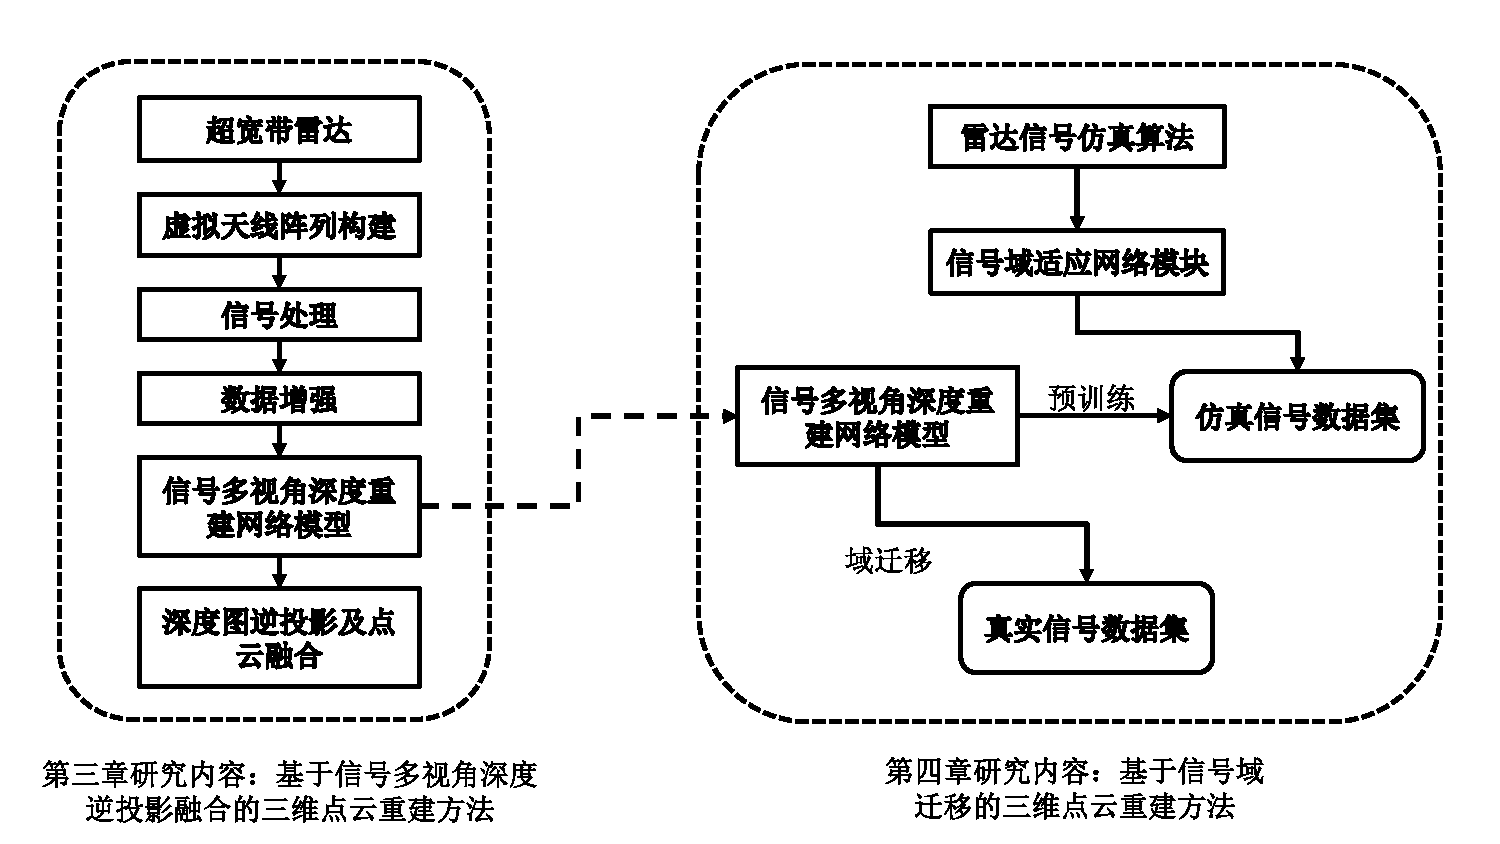
\includegraphics[width=\textwidth]{Figures/研究内容框架.pdf}
    \caption{研究内容框架}
    \label{fig:research_content}
\end{figure}

1）本文提出了一种基于信号多视角深度逆投影融合的三维点云重建方法，该方法利用物体相对超宽带雷达的运动构建出超宽带虚拟阵列，提升了雷达的感知能力，之后对雷达信号进行背景反射消减和有效信号定位，得到去噪后的有效信号；随后针对雷达信号数据集样本单一的问题，本文设计了雷达信号数据增强算法，对雷达数据进行扩充；接着设计了一个从多视角雷达信号到物体多视角深度图的信号多视角深度重建网络模型，并最终通过深度图逆投影和点云融合得到了物体重建三维点云。

2）本文提出了一种基于信号域迁移的三维点云重建方法。针对基于深度学习的三维重建方法存在着的真实雷达信号数据采集耗时、标注费时以及网络模型迁移时训练成本高等问题，本文使用信号域迁移的方法来解决上述问题。本文首先设计并是实现了基于信号建模的雷达信号仿真算法，随后设计了信号域适应网络模块，通过这两个步骤可以合成出一个数据量庞大的仿真信号数据集；随后使用“预训练-微调”的两阶段训练范式将信号多视角深度重建网络模型在仿真信号和真实信号之间进行域迁移，以此提升网络模型在真实信号数据集上的数据效率、训练速度以及性能表现。
\xsection{论文组织结构}{Thesis Organization Structure}
本文总共分为五个章节，各章节具体内容如下：

第一章为绪论部分。首先介绍了本文的研究背景和相关研究的应用价值，接着分析了国内外研究物体三维重建方法的现状，总结了现有方法的不足，并给出了本文的主要贡献和创新点。

第二章为相关理论与技术部分。在第一小节中介绍了脉冲超宽带雷达感知技术，包括脉冲超宽带雷达感知原理以及对应的雷达数据结构；在第二小节中介绍了迁移学习的定义以及应用。

第三章为基于信号多视角深度逆投影融合的三维点云重建方法。首先介绍了超宽带虚拟阵列信号采集与处理流程，随后介绍了雷达信号数据增强算法，接着介绍了信号多视角深度重建网络模型及各模块的设计，之后介绍了深度图逆投影和点云融合流程，最后通过实验评估了本文的三维点云重建方法的性能表现，并且验证了本文方法在物体被遮挡情况下的鲁棒性，同时使用消融实验验证了本文提出的数据增强方法的有效性。

第四章为基于信号域迁移的三维点云重建方法。首先介绍了本文提出的基于信号建模的雷达信号仿真算法，接着介绍了本文设计的信号域适应网络模块；随后详细介绍了信号多视角深度重建网络模型从仿真信号数据集到真实信号数据集的迁移学习步骤，其中还包括了仿真信号数据集的生成方法；最后通过实验评估验证了本文的信号仿真算法和信号域适应网络模块的有效性，以及验证了本文的从仿真域到真实域的迁移学习方法对信号多视角深度重建网络模型的数据效率、训练速度和整体性能的提升。

第五章为结论与展望，主要对本文所做工作做了大致总结，指出主要贡献和创新点；之后对目前工作的不足之处进行分析，对未来工作进行了展望。